\documentclass[12pt]{article}
\usepackage{lingmacros}
\usepackage{tree-dvips}
\usepackage{graphicx} %package to manage images
\usepackage{float}
\graphicspath{ {/} }
\begin{document}

\section*{Creating a Grid}

Our grid relies on several key assumptions. Our grid always assumes that a grid is n x n, and that the start is always at the top left corner and the goal at the bottom right corner. Each tile of the grid has a number on it that respresents the number of tiles you can move in any direction form that grid. Every tile on a grid can go to at least one other tile on the grid.

\begin{figure}[h]
    \centering
    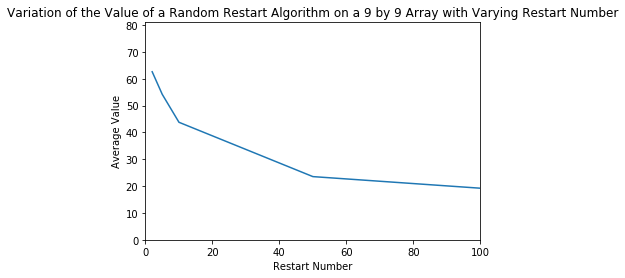
\includegraphics[width=0.9\textwidth]{random_restarts_9x9_restarts}
    \caption{A 5x5 grid with a solution.}
    \label{fig:5x5_solution}
\end{figure}

\section*{Hill Climbing Approach}

The most basic algorithm we tested was a hill-climbing algorithm. This algorithm randomly changes a tile in the grid. If the new value is greater than or equal to the best value of the grid so far, then the change is kept an the hill-climbing algorithm is repeated. Otherwise, the change is discarded. 

\subsection*{Varying Iteration Number}

To measure the effect of iteration number on the output of the hill climbing algorithm, we compared the average final value of grids of differing sizes with different iteration numbers to see what the optimal number of iterations would be for the different sized grids. We tested average final value averaged over 50 runs for iteration numbers of 1,000; 5,000; 10,000; 15,000; and 20,000 for grids of size 5 by 5, 7 by 7, 9 by 9, and 11 by 11.

\begin{figure}[H]
    \centering
    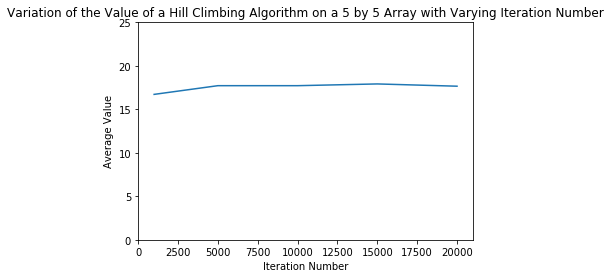
\includegraphics[width=0.9\textwidth]{hill_climbing_5x5_iterations}
\begin{tabular}{ |p{4cm}||p{4cm}|p{4cm}|  }
 \hline
Grid Side Length& Iteration Number &Average Value\\
 \hline
5&1,000&16.72\\
5&5,000&17.72\\
5&10,000&17.72\\
5&15,000&17.92\\
5&20,000&17.66\\
 \hline
\end{tabular}
    \caption{A graph showing the effects of iteration size on final value for a puzzle of size 5 by 5.}
    \label{fig:hill_climbing_5x5_iterations}
\end{figure}

For a 5 by 5 grid, the number of iterations does not seem to make much of a difference, with the largest change being a nominal increase in average value when increasing the iteration number from 1,000 to 5,000. This suggests that the optimal number of iterations that maximizes average value while minimizing computation time is 1,000 iterations for a 5 by 5 grid.

\begin{figure}[H]
    \centering
    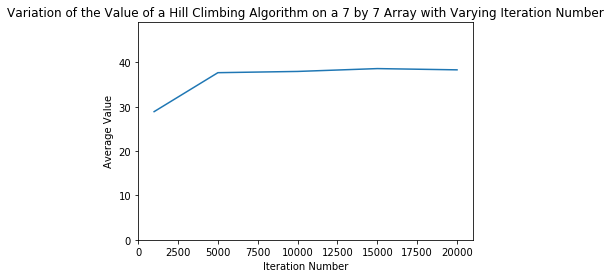
\includegraphics[width=0.9\textwidth]{hill_climbing_7x7_iterations}
\begin{tabular}{ |p{4cm}||p{4cm}|p{4cm}|  }
 \hline
Grid Side Length& Iteration Number &Average Value\\
 \hline
7&1,000&28.88\\
7&5,000&37.66\\
7&10,000&37.94\\
7&15,000&38.58\\
7&20,000&38.30\\
 \hline
\end{tabular}
    \caption{A graph showing the effects of iteration size on final value for a puzzle of size 7 by 7.}
    \label{fig:hill_climbing_7x7_iterations}
\end{figure}

For a 7 by 7 grid, there is a much more marked increase in average value when iteration number increases from 1,000 to 5,000, but once again the average value plateaus as iteration number increases beyond that. This suggests that the optimal number of iterations that maximizes average value while minimizing computation time is 5,000 iterations for a 7 by 7 grid.

\begin{figure}[H]
    \centering
    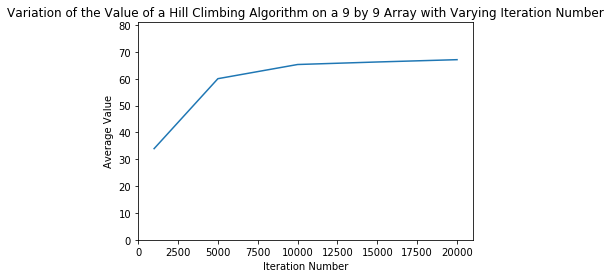
\includegraphics[width=0.9\textwidth]{hill_climbing_9x9_iterations}
\begin{tabular}{ |p{4cm}||p{4cm}|p{4cm}|  }
 \hline
Grid Side Length& Iteration Number &Average Value\\
 \hline
9&1,000&33.96\\
9&5,000&60.02\\
9&10,000&65.30\\
9&15,000&66.24\\
9&20,000&67.10\\
 \hline
\end{tabular}
    \caption{A graph showing the effects of iteration size on final value for a puzzle of size 9 by 9.}
    \label{fig:hill_climbing_9x9_iterations}
\end{figure}

For a 9 by 9 grid, there is a large increase in average value when iteration number increases from 1,000 to 5,000, and another smaller increase when iteration number increases from 5,000 to 10,000. Average value beyond that point increases very slightly. This suggests that the optimal number of iterations that maximizes average value while minimizing computation time is 10,000 iterations for a 9 by 9 grid.

\begin{figure}[H]
    \centering
    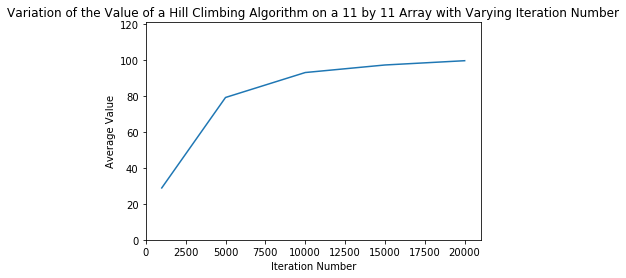
\includegraphics[width=0.9\textwidth]{hill_climbing_11x11_iterations}
\begin{tabular}{ |p{4cm}||p{4cm}|p{4cm}|  }
 \hline
Grid Side Length& Iteration Number &Average Value\\
 \hline
11&1,000&28.86\\
11&5,000&79.20\\
11&10,000&93.08\\
11&15,000&97.28\\
11&20,000&99.66\\
 \hline
\end{tabular}
    \caption{A graph showing the effects of iteration size on final value for a puzzle of size 11 by 11.}
    \label{fig:hill_climbing_11x11_iterations}
\end{figure}



For an 11 by 11 grid, increasing iteration number from 1,000 to 5,000 once again resulted in a steep increase in average value, while subsequent increases in iteration number led to diminishing returns. After 10,000 iterations, subsequent increases in iteration number lead to very small gains. This suggests that the optimal number of iterations that maximizes average value while minimizing computation time is 10,000 iterations for a 11 by 11 grid.



\section*{Hill Climbing with Random Restarts}

The next algorithm we tested was hill-climbing with random restarts. The idea was that a basic hill-climbing algorithm might get stuck at local maxima, where every change would result in a worse grid. In order to circumvent this problem, random restarts would cause the algorithm to start again with a random grid of the same size and run hill-climbing again, repeating the process and keeping track of the best grid.

\subsection*{Varying Restart Number}

All random restart tests were performed with a total of 10,000 iterations. This means that for 2 restarts, there were 5,000 iterations per restart. We tested the effects of having 2, 5, 10, 50, and 100 restarts on grids of size 5 by 5, 7 by 7, 9 by 9, and 11 by 11.

\begin{figure}[H]
    \centering
    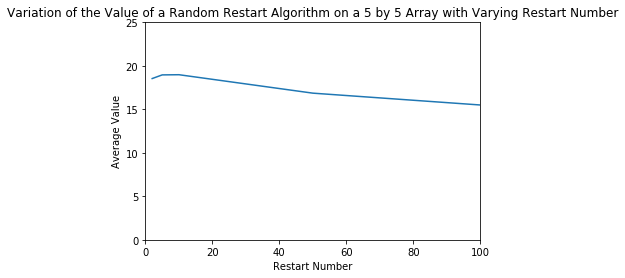
\includegraphics[width=0.9\textwidth]{random_restarts_5x5_restarts}
    \caption{A graph showing the effects of restart number on final value for a puzzle of size 5 by 5.}
    \label{fig:random_restarts_5x5_restarts}
\end{figure}

For a 5 by 5 grid, there is a small increase in average value when restart number increases from 2 to 5, but then average value stays the same until 10 restarts, then plummets. This suggests that the optimal number of restarts for a 5 by 5 grid would be around 2 or 5.

\begin{figure}[H]
    \centering
    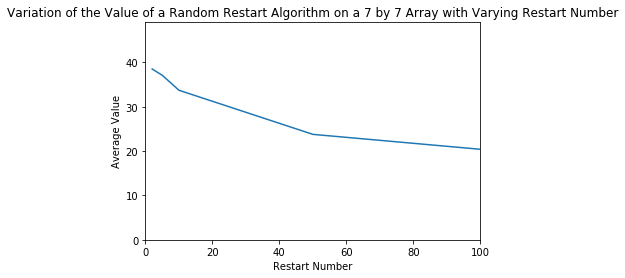
\includegraphics[width=0.9\textwidth]{random_restarts_7x7_restarts}
    \caption{A graph showing the effects of restart number on final value for a puzzle of size 7 by 7.}
    \label{fig:random_restarts_7x7_restarts}
\end{figure}

\begin{figure}[H]
    \centering
    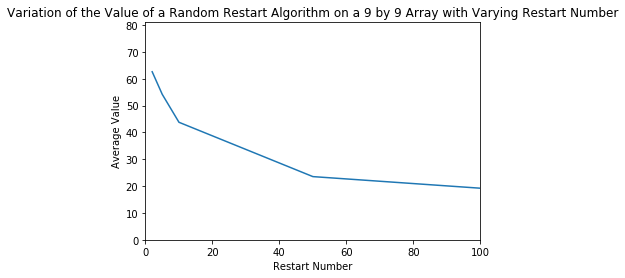
\includegraphics[width=0.9\textwidth]{random_restarts_9x9_restarts}
    \caption{A graph showing the effects of restart number on final value for a puzzle of size 9 by 9.}
    \label{fig:random_restarts_9x9_restarts}
\end{figure}

\begin{figure}[H]
    \centering
    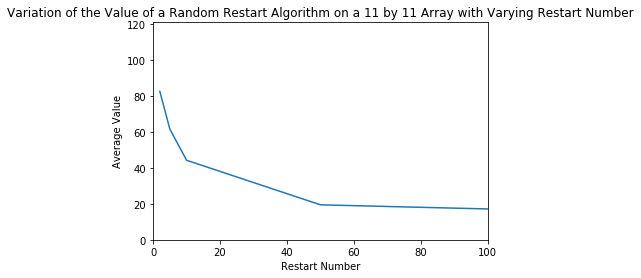
\includegraphics[width=0.9\textwidth]{random_restarts_11x11_restarts}
    \caption{A graph showing the effects of restart number on final value for a puzzle of size 11 by 11.}
    \label{fig:random_restarts_11x11_restarts}
\end{figure}

For grids of larger size, an increase in restart number leads to a decrease in average value, with larger grids leading to a steeper decline. For the hill climbing algorithm, the larger the grid was, the higher the optimal number of iterations was before the average value plateaued. Because an increase from 2 restarts to 5 decreases the number of iterations per restart from 5,000 to just 2,000, this suggests that perhaps there are not enough total iterations for an increase in the number of restarts to outweight the cost of decreasing the number of iterations per restart. For a 5 by 5 grid, which had an optimal iteration number of 1,000, having 5 restarts improved the average value, because having 2,000 iterations per restart was enough to reach the optimal value achievable by a hill climbing algorithm. For an 11 by 11 grid on the other hand, the optimal number of 

\end{document}